\chapter{Risultati}
In questa sezione mostreremo alcuni dei risultati che abbiamo ottenuto, per visualizzarli abbiamo utilizzato
il software ParaView.
All'interno del file \texttt{himod/util/CaseTest.hpp} sono salvati diversi casi test
con soluzione esatta e uno senza (la forzante \`e stata ottenuta usando il symbolic toolbox di Matlab).
Nel caso si fosse interessati ad aggiungere altri casi test \`e possibile aggiungerli modificando i
file \texttt{CaseTest.hpp} e \texttt{CaseTest.cpp}. Una volta creato il caso test 
occorre aggiungerlo allo switch che si trova nella classe \classe{GeneralTest} nella
cartella \texttt{util}. \classe{GeneralTest} \`e una classe che abbiamo sviluppato per poter
lanciare diversi test senza dover modificare il sorgente, ma semplicimente settando 
parametri  e caso test dal datafile di \texttt{GetPot}\footnote{Se si vuole provare a lanciare qualche test si veda il tutorial
\texttt{4\_generaltest}, se invece si vuole vedere come si dovrebbe assemblare un test da zero si veda il tutorial \texttt{1\_ADR} }.
Cominciamo mostrando il caso test senza soluzione esatta, che per\`o \`e pi\`u interessante dal punto di vista qualitativo.
\begin{equation}
 \label{eq:camini}
 \left\{
\begin{aligned}
 &-\Delta u + \vect{\beta}\cdot\nabla u + \sigma u = f &\quad \text{ in }\Omega=(0,2)\times(0,1)\times(0,1)\\
 &u=0 &\quad \text{ su } \Gamma_{in} \cup \Gamma_{lat}\\
 &\nabla u\cdot \vect{n} = 0 &\quad \text{ su } \Gamma_{out},
\end{aligned}
\right.
\end{equation}
dove $\vect{\beta}=(5,1,0)$, $\sigma=0.3$ e $f$ \`e riportata in figura \ref{fig:fcamini}.
In figura \ref{fig:confrontocamini} abbiamo sulla sinistra la soluzione ottenuta con 
gli elementi finiti (sempre con LifeV), utilizzando una griglia strutturata con \# elementi in direzione $x$
e \# in direzione $y$ e $z$, sulla destra invece c'\`e la soluzione ottenuta con HiMod, \# elementi in direzioni $x$
e 50 modi. Osserviamo che 50 modi, in un problema come questo dove la geometria e le condizioni al bordo sono le stesse in direzione
$x$ e $y$, significa circa 7 modi in direzione $y$ e altrettanti in direzione $z$.
Vediamo come, dal punto di vista qualitativo, il fenomeno venga colto bene anche dalla riduzione gerarchica di modello.
Nella figura \ref{fig:camini2d+} vediamo diverse sezioni trasversali del dominio e possiamo apprezzare, sempre dal punto di vista qualitativo,
la convergenza. Vediamo che gi\`a con 9 modi la soluzione \`e ragionevole anche se non \`e in grado di cogliere 
bene tutte le caratteristiche della soluzione, con 16 modi ci sono evidenti miglioramenti e con 25 siamo gi\`a a convergenza dal punto di 
vista qualitativo, non abbiamo quindi riportato risultati con pi\`u di 25 modi.
Infine, in figura \ref{fig:camini2D}, riportiamo un'altra visualizzazione di una sezione orizzontale con $y=0.5$.
Anche qui possiamo apprezzare la convergenza.
Nei successivi esperimenti abbiamo testato diverse combinazioni di dati al bordo e abbiamo cercato di verificare la convergenza del 
metodo. 
\subsection*{Convergenza}
Dal punto di vista teorico la teoria della convergenza per le basi istruite \`e ancora in fase di sviluppo.

Nel caso 2D si ha una convergenza di ordine due in $L^2(\Omega)$ rispetto al numero di modi.
In particolare nel caso Dirichlet in 2D usando i P1 in direzione $x$ si ha per $u\in H^2(\Omega)$
\begin{equation}
 \label{eq:stimainl2}
 ||u-u_{m,h}||_{L^2(\Omega)}\leq C ( h^2+m^{-2}) ||u||_{H^2},
\end{equation}
per maggiori dettagli su questo caso si possono trovare in \cite{zilio:himod} teoremi 3.15 e 3.16.

In 3D tenendo conto che $m\sim m_y\cdot m_x$ e con altre considerazioni basate sulle propriet\`a del problema agli autovalori
\`e ragionevole aspettarsi un ordine uno in $L^2(\Omega)$ rispetto al numero di modi, ma la dimostrazione 
non \`e stata ancora terminata.

Nella figura \ref{fig:ddddconv} possiamo vedere un caso test con condizioni di Dirichlet sul bordo laterale. Vediamo 
come l'ordine di convergenza sia pari a uno. Vediamo anche che se si usa una griglia elementi finiti troppo 
lasca ad un certo punto l'errore non decresce pi\`u al crescere del numero di modi, perch\`e 
l'errore elementi finiti \`e superiore a quello di modello dovuto all'approssimazione modale.
Vediamo per\`o che riducendo il passo della griglia le curve dell'errore si attestano tutte sulla stessa linea.
Nel caso riportato in figura \ref{fig:drdrconv} abbiamo un caso test con condizioni miste sui lati del quadrato:
il lato in basso e in alto hanno condizioni di Dirichlet, mentre i lati a destra e a sinistra hanno condizioni di Robin.
Anche qui possiamo vedere come il grafico di convergenza confermi i risultati attesi dalla teoria.
Infine abbiamo costruito un caso test con condizioni di Robin su tutti i lati. In figura \ref{fig:rrrr_conv} possiamo 
vedere come l'ordine di convergenza sembra essere superiore alla velocit\`a attesa, questo comportamento in realt\`a 
si verifica anche nei casi test bidimensionali con condizioni al bordo di Robin, dal punto di vista teorico ancora non ci sono 
spiegazioni convincenti, tuttavia questo comportamento si verifica puntualmente.

Abbiamo poi riportato alcuni test per cercare di confrontare gli elementi finiti con HiMod.
In figura \ref{fig:dof} abbiamo riportato il numero di gradi di libert\`a dei due metodi lungo la slice trasversale utilizzati per 
approssimare il caso test con condizioni di Dirichlet che abbiamo utilizzato anche per osservare la convergenza.
Per gli elementi finiti abbiamo utilizzato una griglia strutturata e entrambi i metodi condividono la stessa griglia 
in direzione $x$. Sull'asse delle ordinate abbiamo riportato l'errore in norma $L^2(\Omega)$.
Si vede come a parit\`a di precisione, con himod sia possibile ottenere utilizzare molti meno gradi di libert\`a in direzione trasversale.
Tuttavia questo dipende anche dal caso test, perch\`e l'ordine di convergenza \`e lo stesso, quindi tutto dipende dalla 
costante davanti alla stima dell'errore. \`E chiaro che se la soluzione non presenta dinamiche particolarmente complesse in direzione trasversale,
se la base scelta \`e buona gi\`a con i primi modi si potranno cogliere le caratteristiche principali e dunque la curva HiMod
in figura \ref{fig:dof} si trover\`a al di sotto della curva per gli elementi finiti.

Infine, sempre sul caso test con condizioni di Dirichlet, abbiamo cercato di capire quanto tempo impiega l'assemblaggio della matrice
rispetto all'analogo test assemblato con il pacchetto \texttt{ETA} di \texttt{LifeV}.
I risultati si possono vedere in figura \ref{fig:time} e vediamo come, a parit\`a di precisione, il tempo di assemblaggio 
della matrice sia minore che nel caso elementi finiti, ci\`o \`e dovuto al minor numero di gradi di libert\`a.

% \begin{itemize}
% \item Introduzione teorica
% \item Osservazione sull'influenza dell'errore fem (particolare nel caso RRRR sarebbe da verificare)
% \item Notare la superconvergenza (come da teoria?)
% \end{itemize}
% 
% % \begin{figure}[!htbp]
% %         \centering%
% %         \subfigure[DDDD]%
% %           {\label{fig: convDDDD}\includegraphics[scale=0.25]{Convgopergenze/DDDD_ADR.eps}}\qquad
% %         \subfigure[DRDR]%
% %           {\label{fig:convDRDR}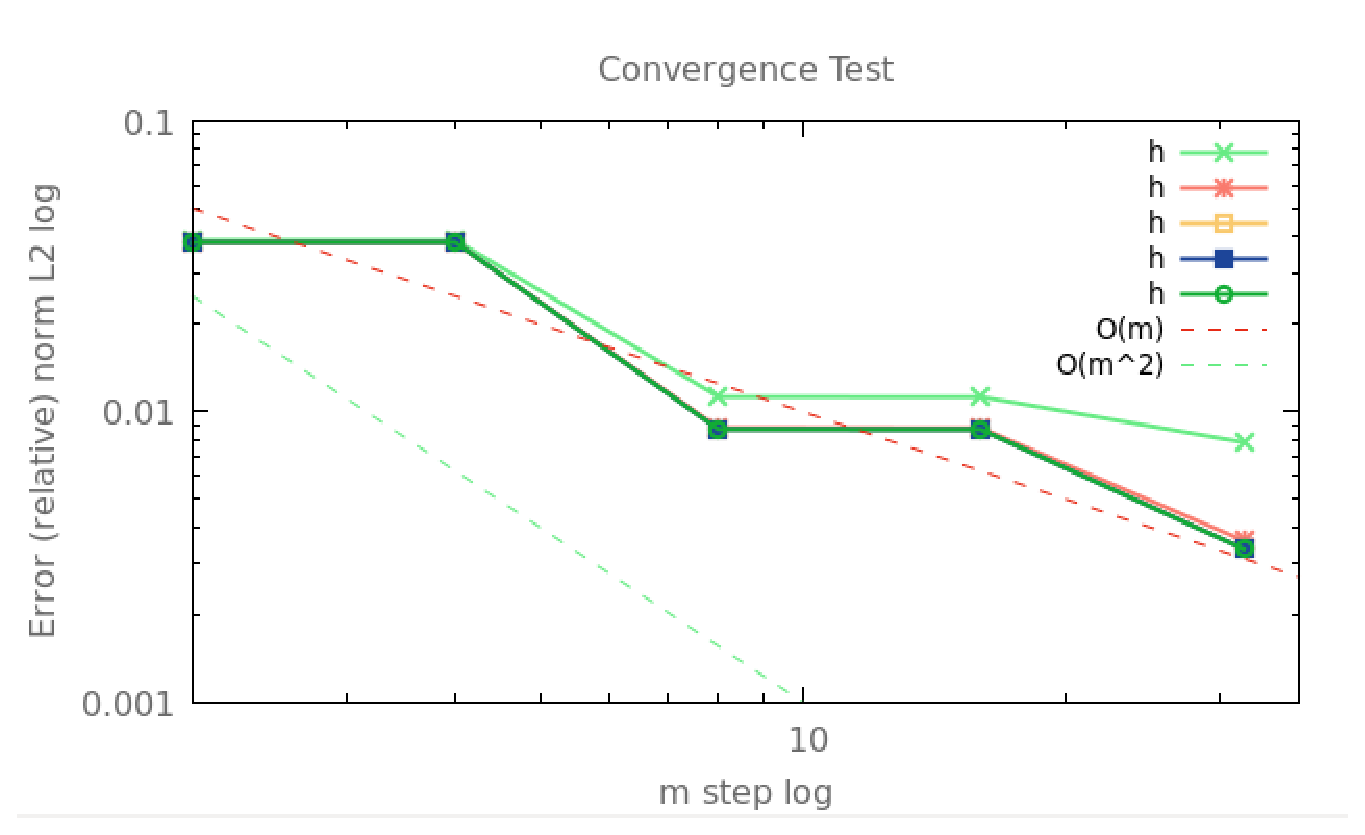
\includegraphics[scale=0.25]{Convergenze/DRDR.eps}}\qquad
% % 		\subfigure[RRRR]%
% %           {\label{fig:convRRRR}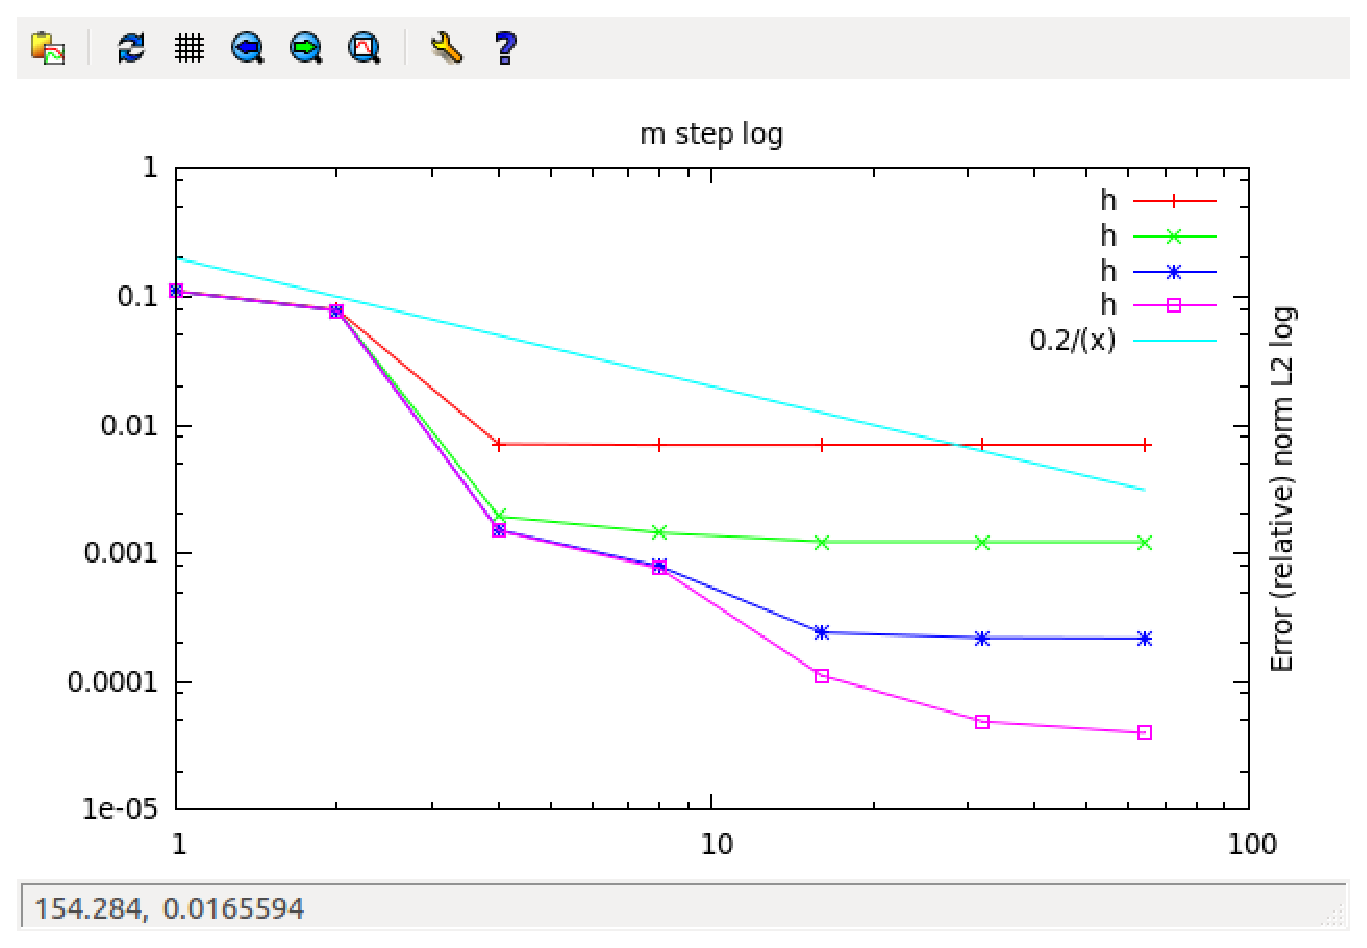
\includegraphics[scale=0.25]{Convergenze/RRRR.eps}}\qquad
% %         \label{fig: convergenze}
% %         \caption{Convergenze casi test}
% % \end{figure}
% 
% \begin{itemize}
% \item Confronto gradi di libert\`a spesi e errore norma L2
% \item Tempo di assemblaggio problema
% \end{itemize}
% \begin{figure}[!h]
% \centering
%           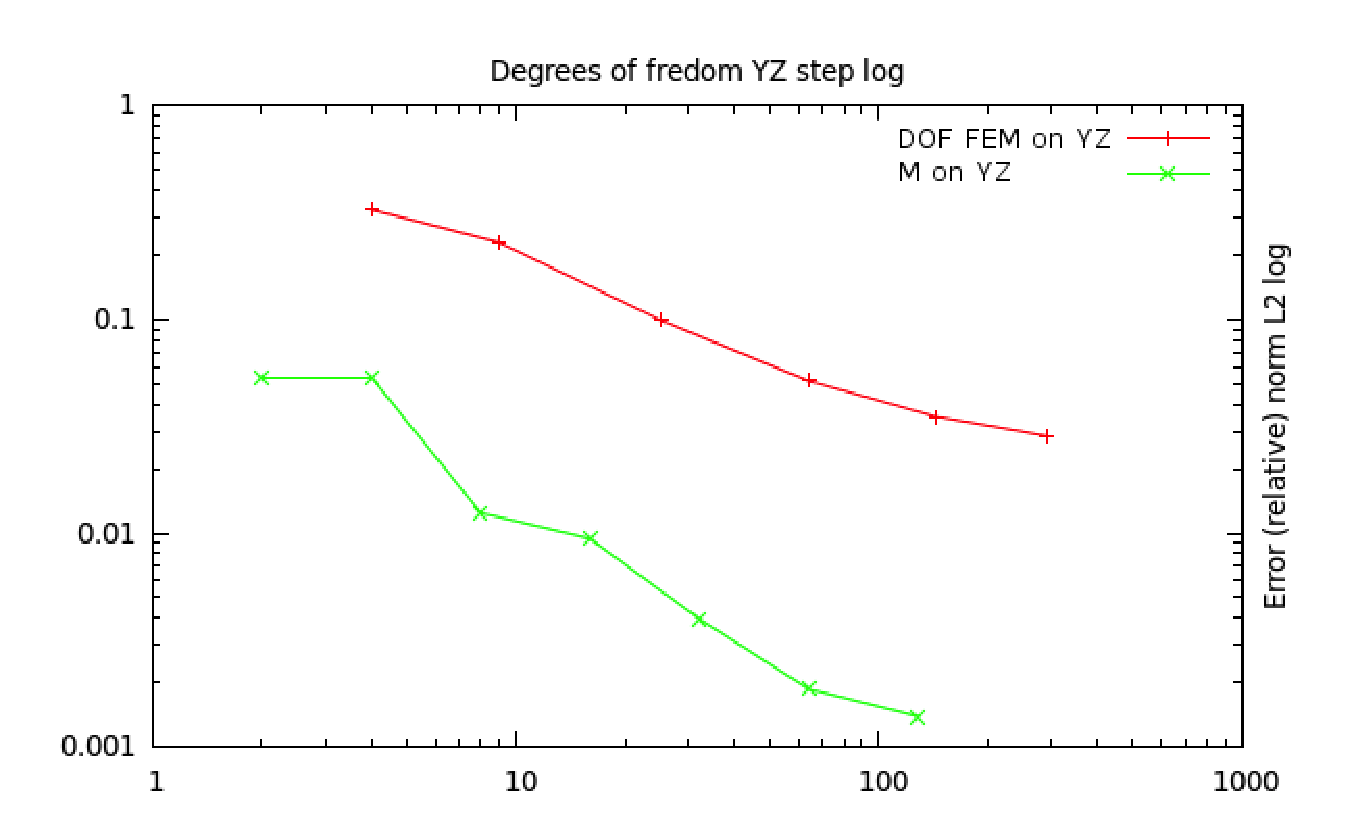
\includegraphics[scale=0.25]{Convergenze/ConfrontoDOF.eps}\qquad
%         \caption{ Confronto DOF}
%         \label{fig: Confronto DOF}
% \end{figure}
% 
% \begin{figure}[!h]
% \centering
%           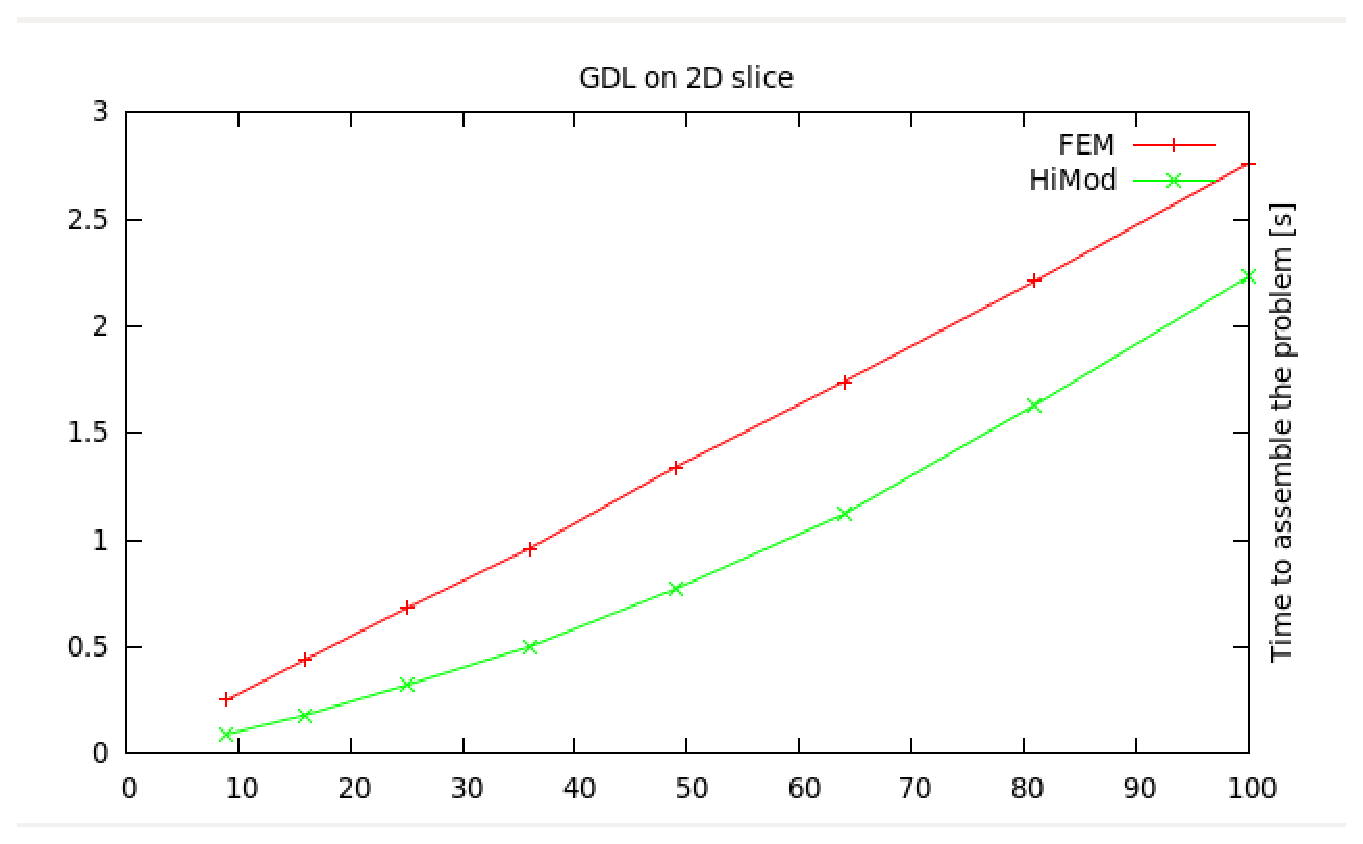
\includegraphics[scale=0.25]{Convergenze/Confronto_tempi.eps}\qquad
%         \caption{ Confronto tempi assemblaggio}
%         \label{fig: Confronto tempi}
% \end{figure}
% 
% \begin{itemize}
% \item Presentazione del caso test
% \item Osservazione sull'aggiunta progressiva di modi (sempre pi\`u frequenze vengono considerate e l'approssimazione cresce)
% \item Commento sui risultati 3D
% \end{itemize}
% 
% \begin{figure}[!htbp]
%         \centering%
%         \subfigure[m=9.]%
%           {\label{fig: slice9}\includegraphics[scale=0.15]{DDDD_ADR/HiMod9slice.eps}}\qquad
%         \subfigure[m=16.]%
%           {\label{fig:slice16}\includegraphics[scale=0.15]{DDDD_ADR/HiMod16slice.eps}}\qquad
% 		\subfigure[m=25.]%
%           {\label{fig:slice25}\includegraphics[scale=0.15]{DDDD_ADR/HiMod25slice.eps}}\qquad
%           \subfigure[FEM.]%
%           {\label{fig:sliceFEM}\includegraphics[scale=0.15]{DDDD_ADR/FEMslice.eps}}\qquad
%         \caption{Caso test DDDD sezione XZ}
%         \label{fig:DDDD_ADR slice}
% \end{figure}
% 
% \begin{figure}[!htbp]
%         \centering%
%                 \subfigure[Forzante e trasporto.]%
%           {\label{fig: force term}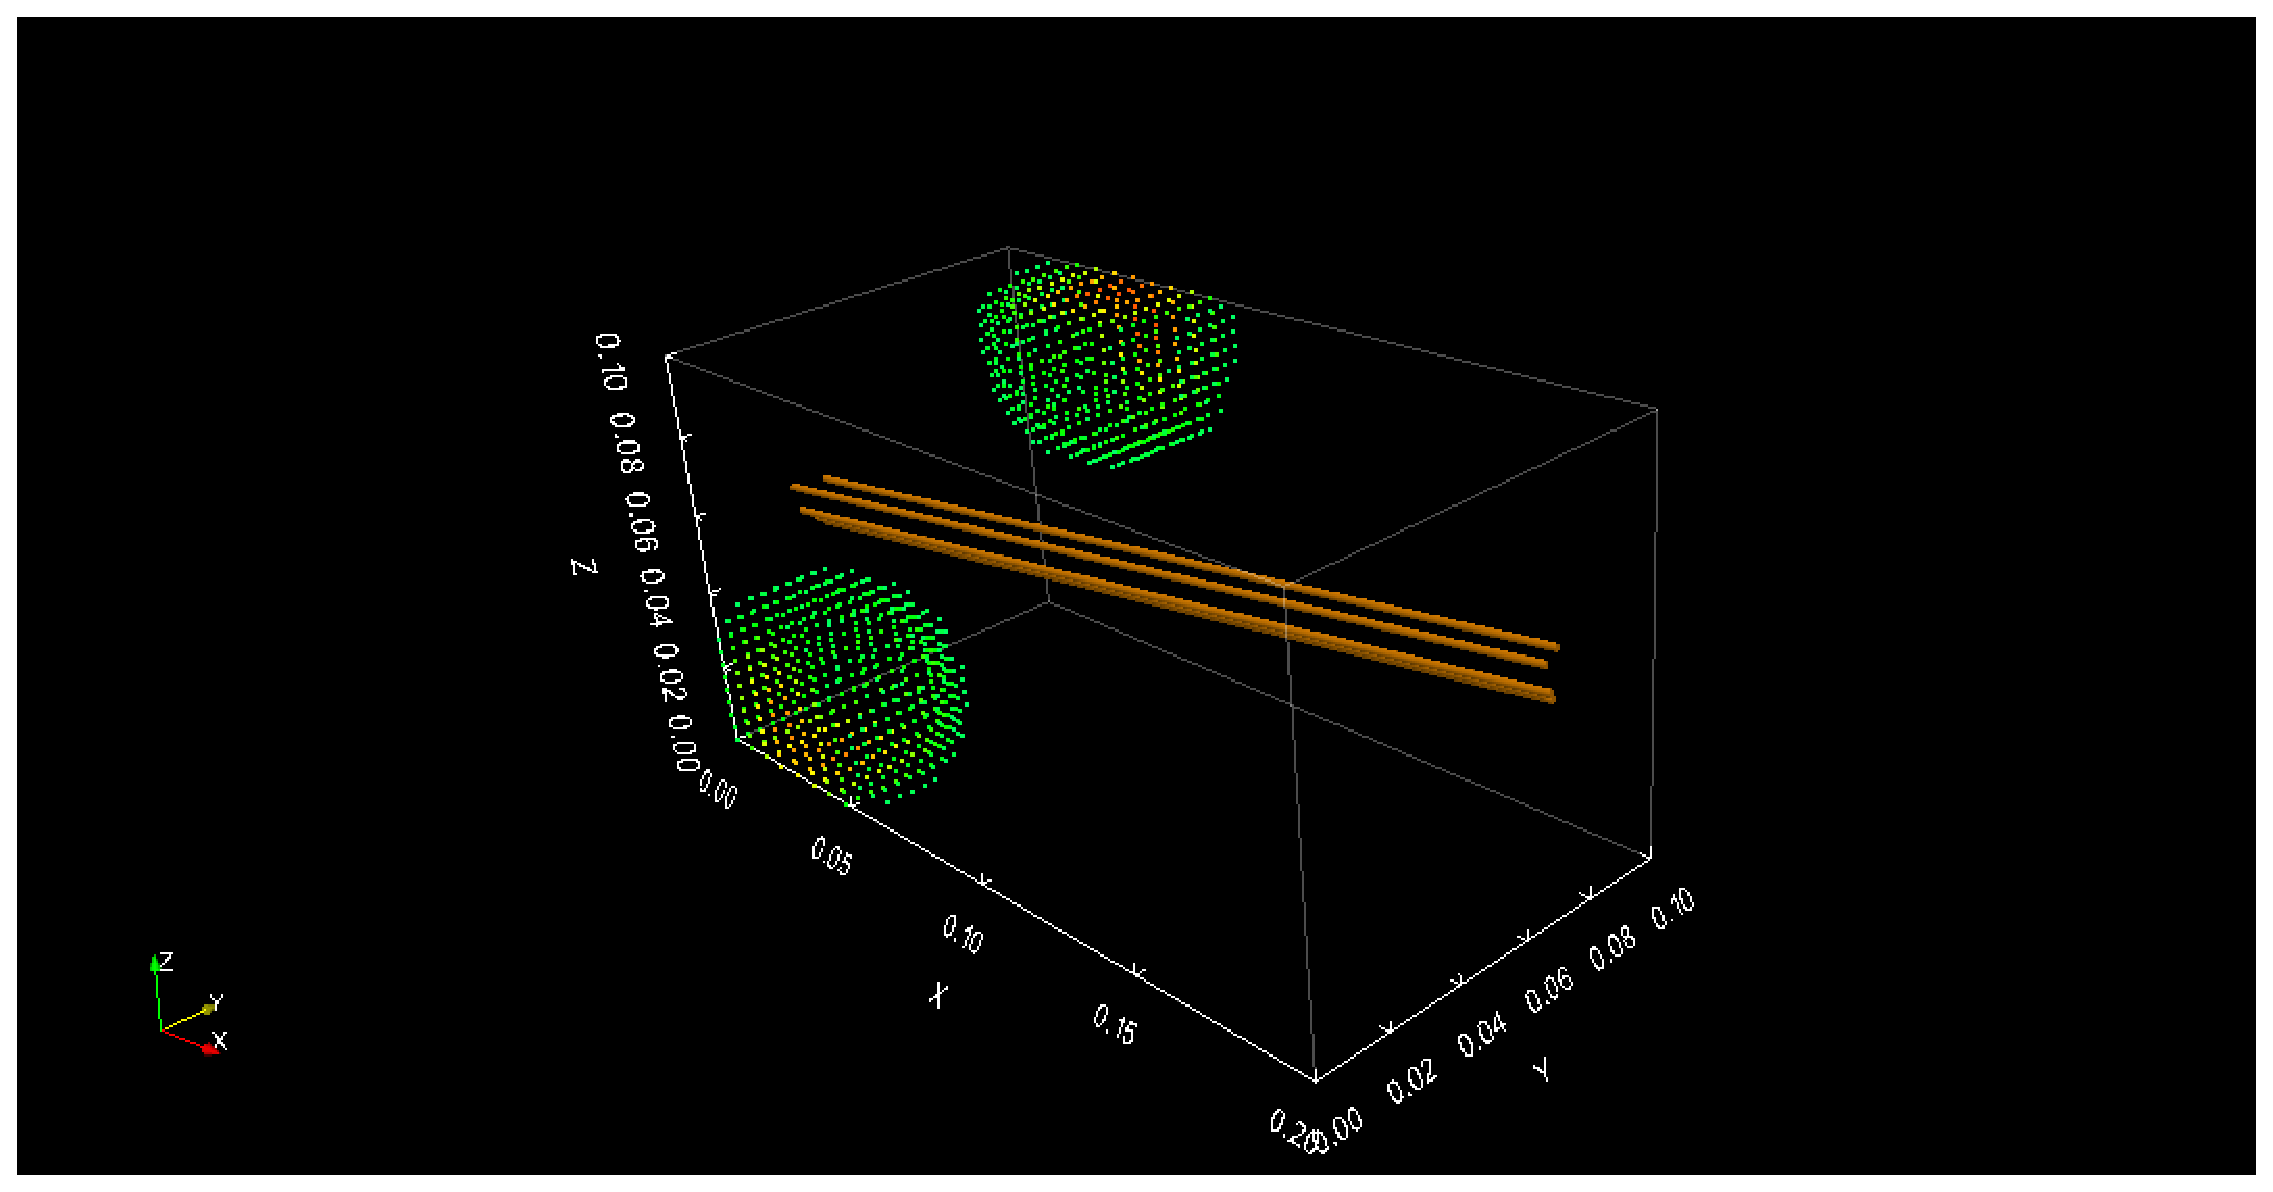
\includegraphics[scale=0.36]{DDDD_ADR/ForcetermTrasport.eps}}\qquad
%         \subfigure[Soluzione FEM.]%
%           {\label{fig: FEMsol}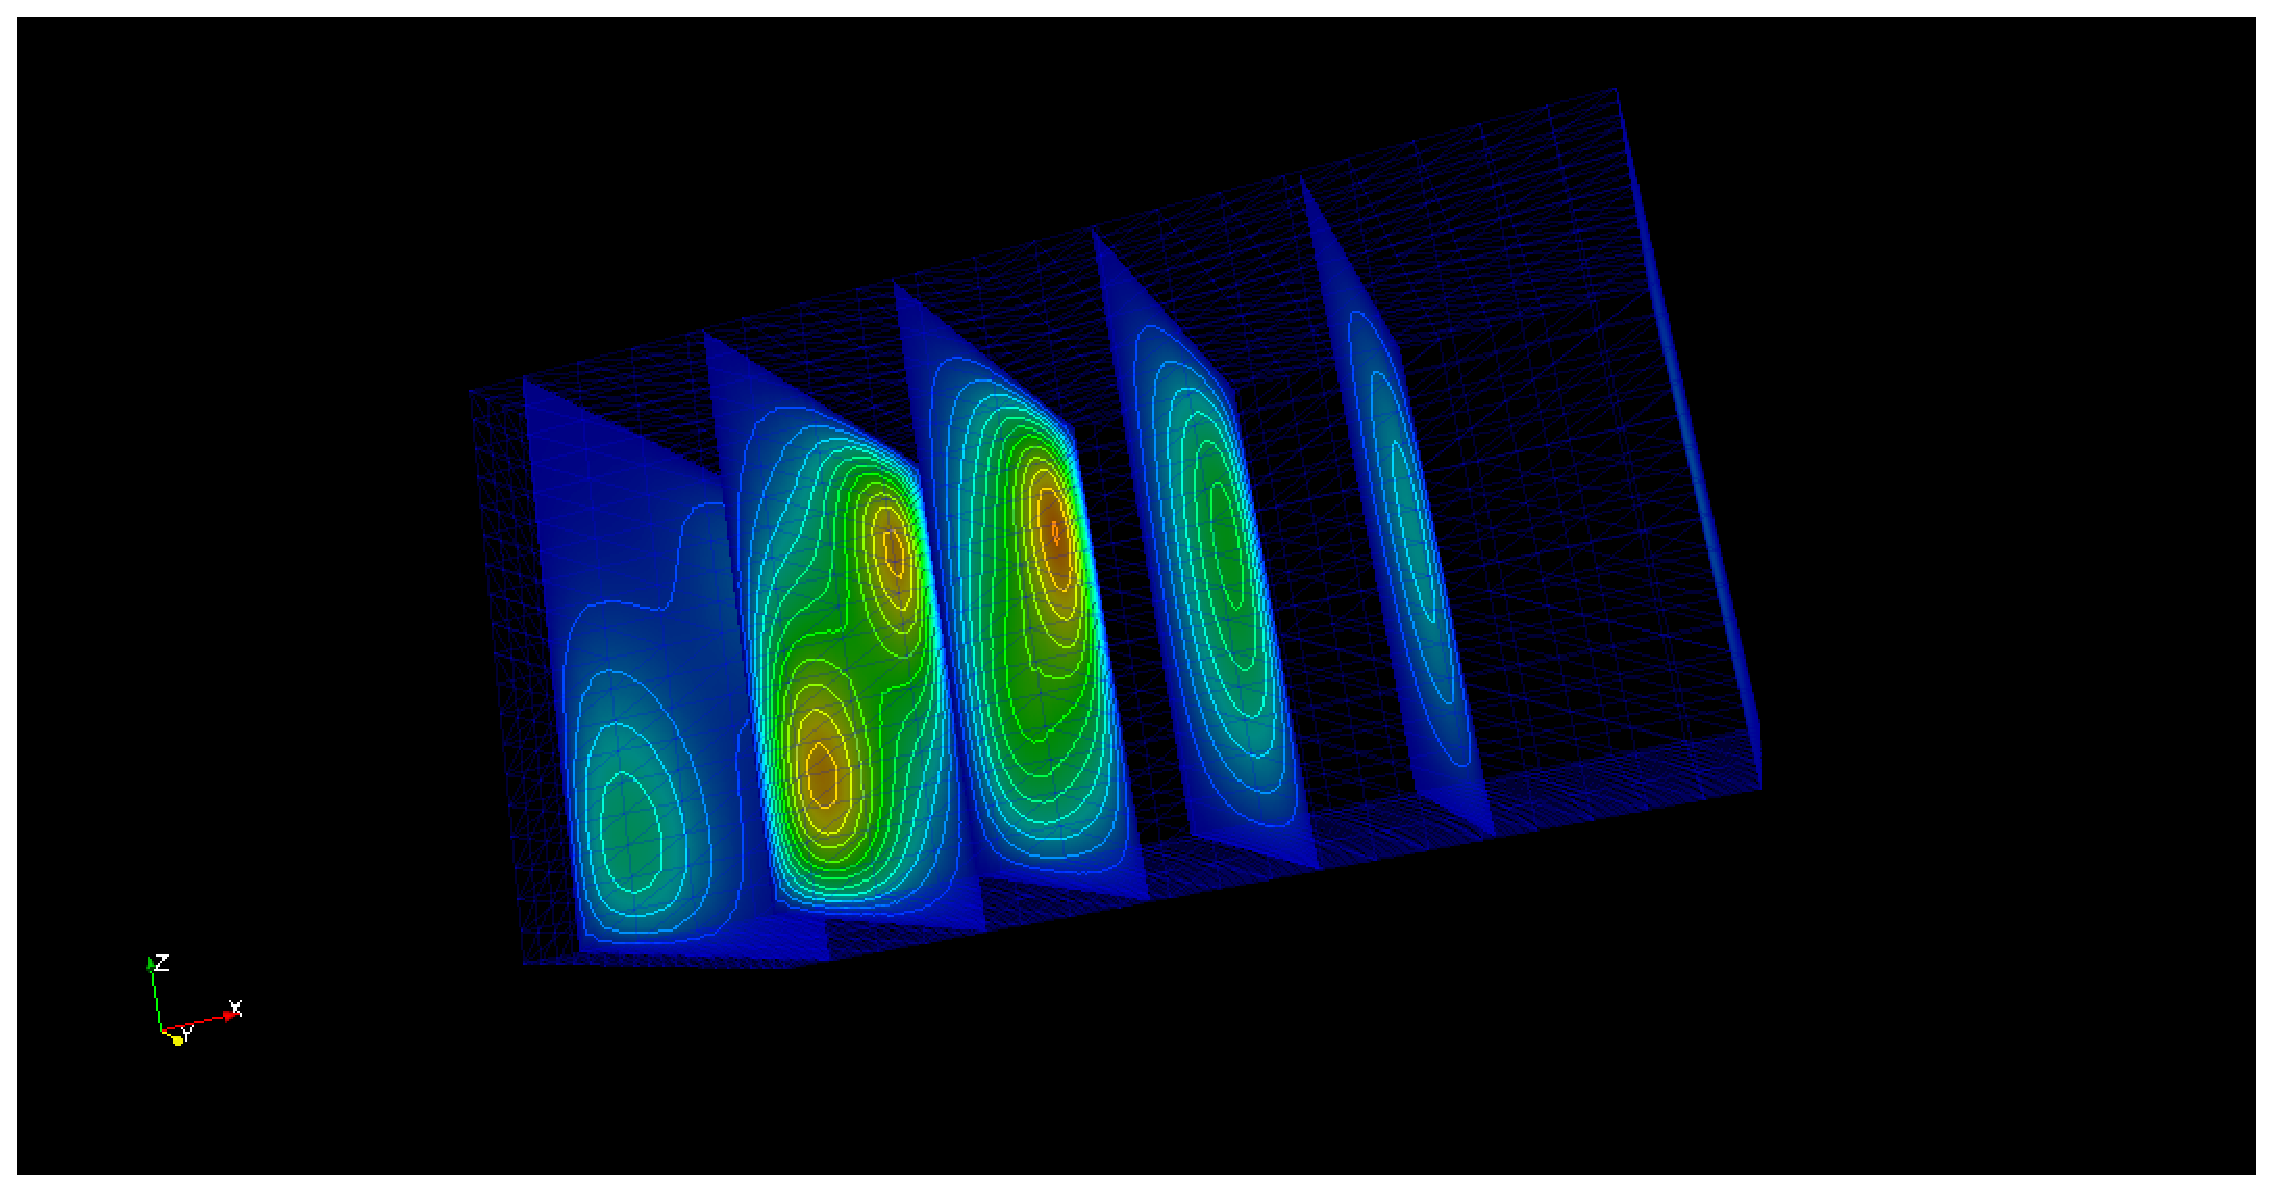
\includegraphics[scale=0.36]{DDDD_ADR/FEM.eps}}\qquad
%         \subfigure[Soluzione HiMod m=50.]%
%           {\label{fig:HiMod50sol}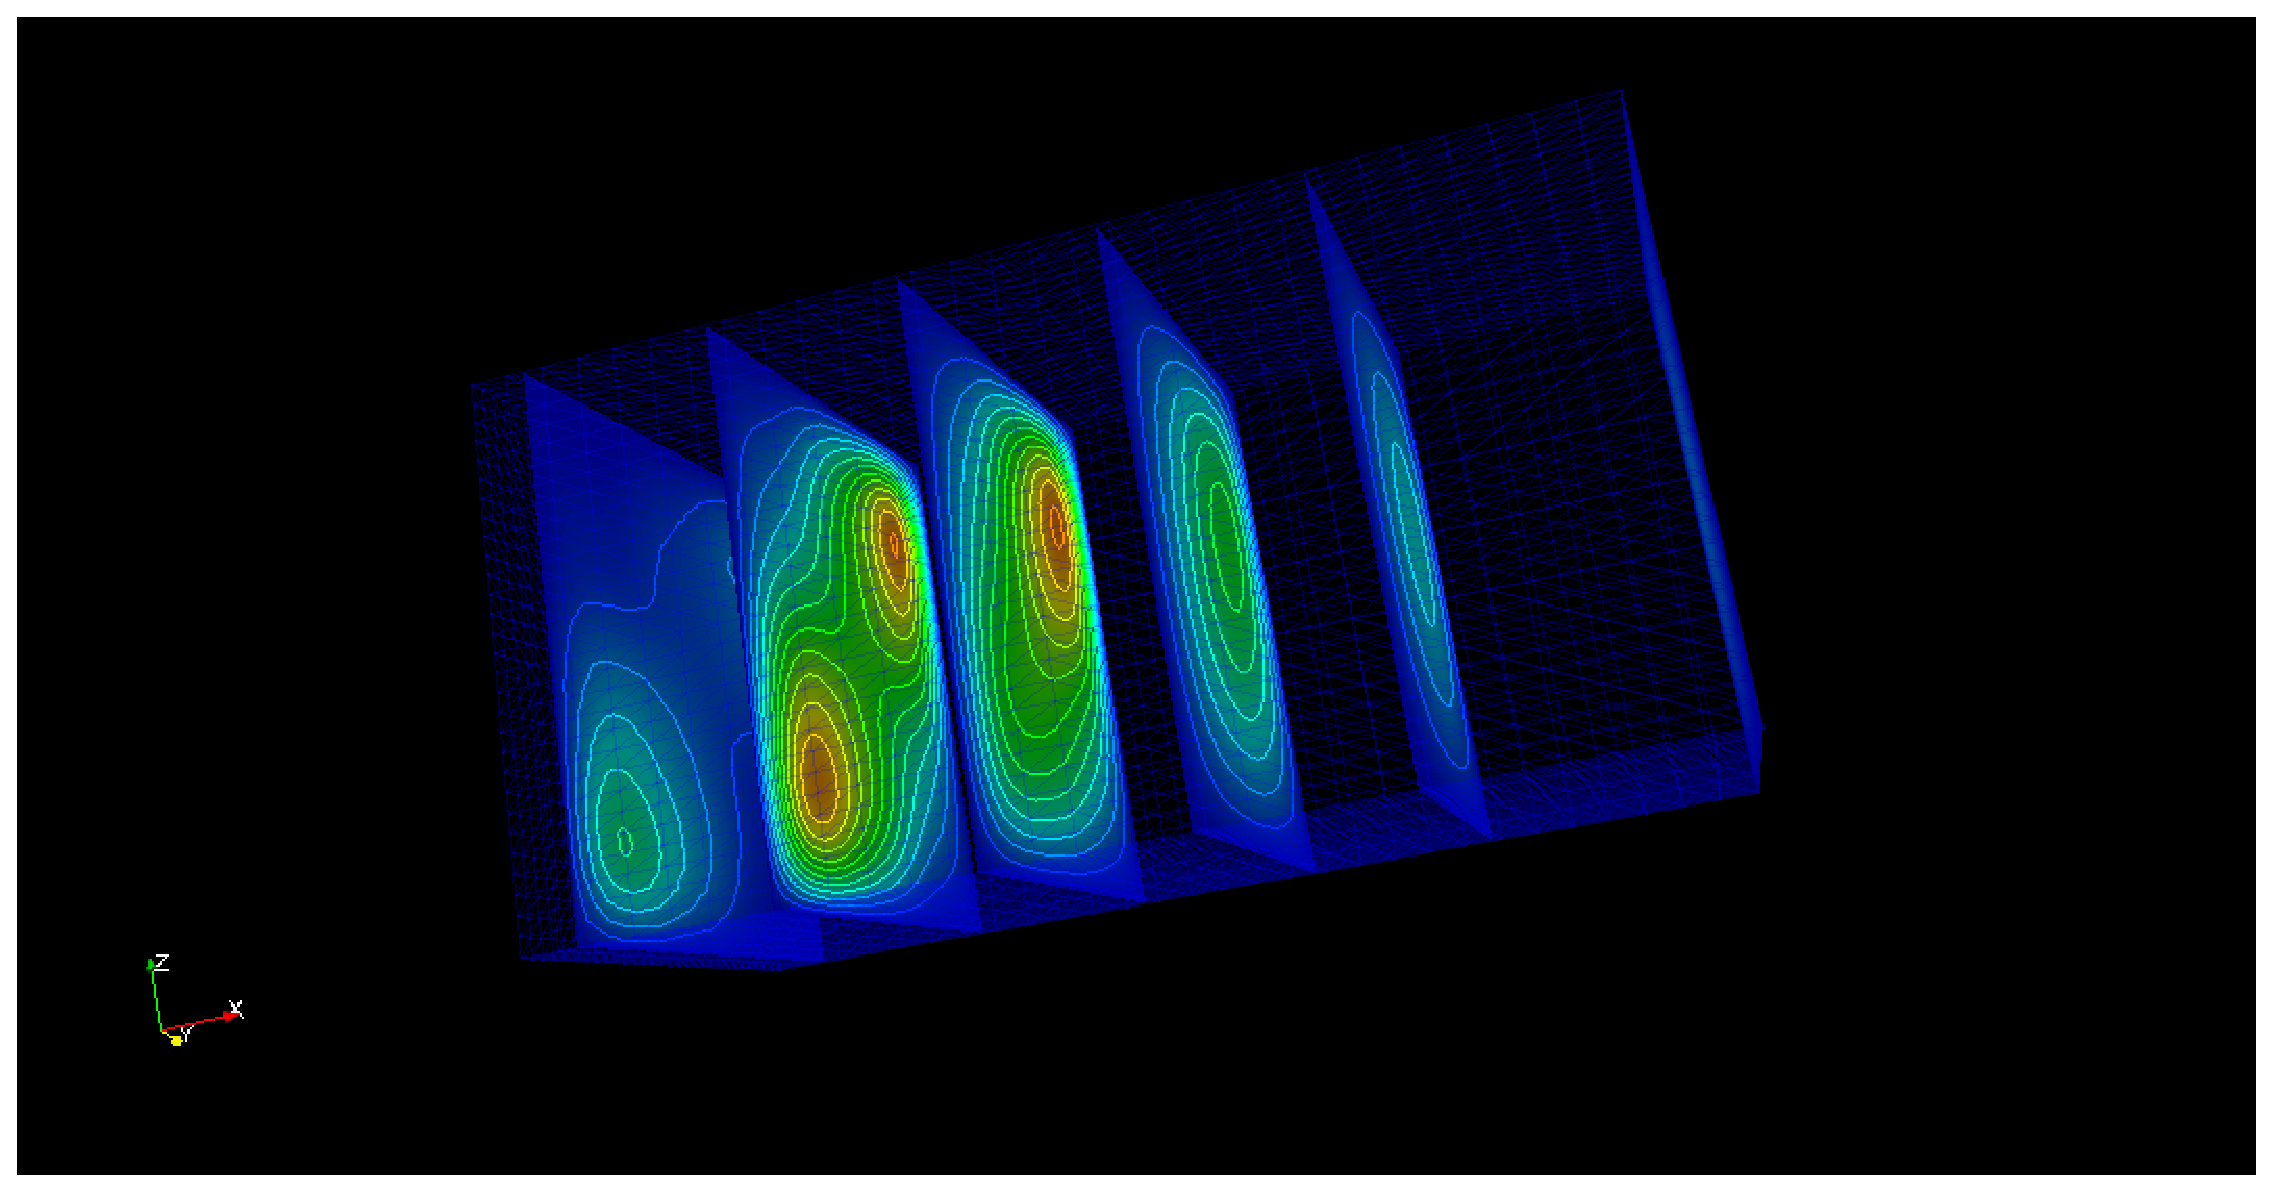
\includegraphics[scale=0.36]{DDDD_ADR/HiMod50.eps}}\qquad
%         \caption{Caso test DDDD\_ADR}
%         \label{fig:DDDD_ADR}
% \end{figure}